\documentclass[lang=cn, zihao=4.5]{elegantbook}
\usepackage{hyperref}
\usepackage{booktabs}

% font settings
\definecolor{mgreen}{RGB}{0,166,82}

% watermark settings
%\usepackage{ctex, draftwatermark, everypage}
%	\SetWatermarkText{DEEP Team 讲义模版}
%	\SetWatermarkLightness{0.95}
%	\SetWatermarkScale{0.3}

% customised commands
\newcommand{\xl}[1]{\overrightarrow{#1}}
\newcommand{\nd}[1]{〔#1〕}
\newcommand{\ssb}[1]{\left( #1 \right)}
\newcommand{\R}{\mathbb{R}}
\newcommand{\C}{\mathbb{C}}
\newcommand{\F}{\mathbb{F}}
\newcommand{\sw}[1]{\boxed{\text{解法 #1}} \ }
\newcommand{\buzhou}[1]{$#1^{\circ} \ $}
\usepackage{ulem}
	\newcommand{\tk}{\uline{\hspace{4em}}}
\newcommand{\pspace}{\vspace{0.5em}}
\usepackage{amsmath,amsfonts}
	\DeclareMathOperator{\spn}{span}
	\DeclareMathOperator{\ic}{i}
	\DeclareMathOperator{\card}{card}
	\DeclareMathOperator{\arccot}{arccot}
	\DeclareMathOperator{\setjianfa}{\textbackslash}
\newcommand{\examplefont}[1]{\color{mgreen} \textbf{#1}}

% cover settings

\title{高中数学}

\author{Johnny Tang}
\institute{DEEP Team}
\date{January 21, 2023}

\extrainfo{请:相信时间的力量,敬畏概率的准则}


\cover{cover.png}

% 本文档命令


% 修改标题页的橙色带
% \definecolor{customcolor}{RGB}{32,178,170}
% \colorlet{coverlinecolor}{customcolor}


\begin{document}

\maketitle

\frontmatter

\mainmatter

\tableofcontents

注:初等数论部分在我学完后开始编写.

\newpage

\part{预备知识}

\setcounter{chapter}{-1}
\chapter{数理逻辑与集合}

\section{数理逻辑}

\subsection{命题的概念}

\begin{definition}{命题}
	由一个陈述句表达的、具有真值的判断称为\textbf{命题}.
\end{definition}
\begin{remark}
	有一种特殊的命题,形如“若$p$,则$q$”,这种命题可以帮助我们判断很多要素.
\end{remark}

命题之间有一些特殊关系.

\begin{definition}{充分条件与必要条件} %ayumu数分p1定义0.1
	设命题$A$和$B$.若$A$可以推得$B$,则称命题$A$是$B$的\textbf{充分条件}(sufficient condition),$B$是$A$的\textbf{必要条件}(necessary condition),记作$$A \Rightarrow B,~\text{或}~B \Leftarrow A$$
	若$A$可以推得$B$且$B$可以推得$A$,则称命题$A$和$B$互为\textbf{充分必要条件}(necessary and sufficient condition),简称充要条件,此时也称命题$A$和$B$等价($A$成立当且仅当$B$成立),记作$$A \Leftrightarrow B$$
	此时$B \Rightarrow A$的过程称为充分性,$A \Rightarrow B$的过程称为必要性.
\end{definition}
\begin{remark}
	还有一个类似的逻辑语言:有且仅有(恰有),这意味着存在一个(存在性)且只有一个(唯一性).例如,平面中,过直线外一点有且仅有一条直线与之平行.
\end{remark}

可以用图像来更好理解该定义.

\begin{figure}[h!]
	\centering
	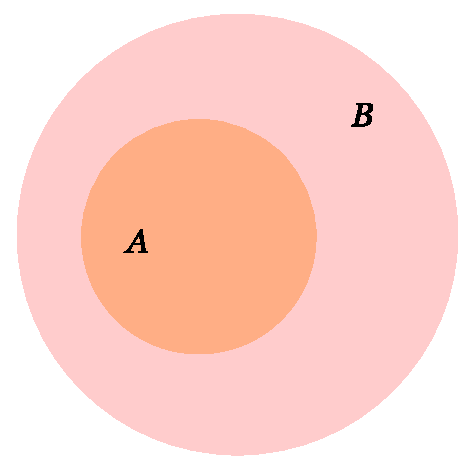
\includegraphics[width=5cm]{attachment/202302191.pdf}
	\caption{例如,此时$A$是$B$的必要且不充分条件}
\end{figure}

\begin{example}
	(1)一个四边形“是菱形”是“它的对角线互相垂直”的\tk 条件. \\
	(2)“$0<x<1$”是“$x<2$”的\tk 条件. \\
	(3)设有命题$p,q$.则“$p \Rightarrow q$”是“$p \Leftrightarrow q$”的\tk 条件. \\
	(4)“$x^2-5x+6 \neq 0$”是“$x \neq 2$”的\tk 条件.
\end{example}
\begin{solution}
	(1)充分且不必要;(2)充分且不必要;(3)必要且不充分;(4)必要且不充分.
\end{solution}

不过这种直观的判断方式比较迷惑,我们可以通过命题的逻辑运算更好地思考这些问题.

\begin{definition}{命题的逻辑运算} %ayumu数分p1定义0.3
	设命题$A$与$B$, \\
	(1)若$A$和$B$中至少有一个命题成立,则称$A$\textbf{或}(or)$B$,记作$$A \vee B$$
	(2)若$A$和$B$同时成立,则称$A$\textbf{且}(and)$B$,记作$$A \wedge B$$
	(3)若$A$的相反形式成立,则称\textbf{非}(not)$A$(或称$A$的否定),记作$$\neg A$$
\end{definition}
\begin{remark}
	关于“且”“或”的否定,存在如下规律:
	$$\neg (A \vee B) = (\neg A) \wedge (\neg B)$$
	$$\neg (A \wedge B) = (\neg A) \vee (\neg B)$$
\end{remark}

另外,对于任意命题的否定,有一个重要法则.在二值逻辑中,该定律实际上告诉我们一个命题$P$要么为真、要么为假.

\begin{proposition}{排中律}
	对于任何命题$P$,$P \vee (\neg P)$为真.
\end{proposition}

\begin{definition}{存在,任意}
	设命题$A$, \\
	(1)若\textbf{存在}(exist)$x$使得命题$A$成立,可以记作$$\exists x~s.t.~A$$
	(2)若对于\textbf{任意}(for all)$x$都能使得命题$A$成立,可以记作$$\forall x,A$$
\end{definition}
\begin{remark}
	“$s.t.$”是“\textit{such that}”的缩写.
\end{remark}
\begin{remark}
	“存在”与“任意”的否定如下:
	$$\neg (\forall x,A) = \exists x~s.t.~\neg A$$
	$$\neg (\exists x~s.t.~A) = \forall x,\neg A$$
\end{remark}

\subsection{特殊的命题}

我们可以对特殊的“若$p$,则$q$”型命题进行更进一步的讨论.

\begin{definition}{原命题,逆命题,否命题,逆否命题}
	设有\textbf{原命题}(primitive proposition)可以表示为$P \Rightarrow Q$的形式. \\
	(1)\textbf{逆命题}(converse proposition)定义为:$$Q \Rightarrow P$$
	(2)\textbf{否命题}(inverse proposition)定义为:$$\neg P \Rightarrow \neg Q$$
	(3)\textbf{逆否命题}(contrapositive proposition)定义为:$$\neg Q \Rightarrow \neg P$$
\end{definition}
\begin{remark}
	此时否命题就是原命题的否定形式,即$\neg (P \Rightarrow Q) = (\neg Q \Rightarrow \neg P)$.
\end{remark}

回顾上一个例题的最后一问,除了用直观的判断方式以外,我们还可以用反证法说明“若$x \neq 2$,则$x^2-5x+6 \neq 0$”.实际上,反证法的本质就是以下命题所述:

\begin{proposition}
	逆否命题与原命题的真假性相同.
\end{proposition}

这个命题也可用图像来解释:

\begin{figure}[h!]
	\centering
	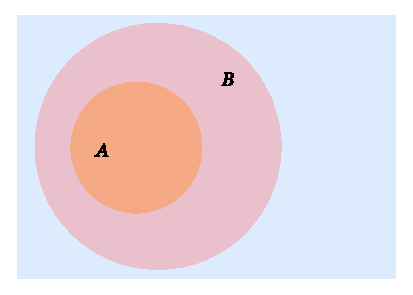
\includegraphics{attachment/202302192.pdf}
	\caption{逆否命题与原命题的真假性比较}
\end{figure}

容易发现,其中“若$A$,则$B$”就等价于“若$\neg B$(即矩形除去大圆的区域),则$\neg A$(即矩形除去小圆的区域)”.




\begin{example}
	证明:$\sqrt{2}$是无理数.
\end{example}
\begin{proof}
	设原命题:“所有能表示为$\dfrac{p}{q}~$($p,q$都是正整数且互质)的形式的数都是有理数”$\Rightarrow$“$\sqrt{2}$是无理数”. \\
	则原命题等价于“所有不能表示为$\dfrac{p}{q}~$($p,q$都是正整数且互质)的形式的数都是无理数”$\Rightarrow$“$\sqrt{2}$是无理数”. \\
	构造逆否命题:“$\sqrt{2}$是有理数”$\Rightarrow$“存在一个不能表示为$\dfrac{p}{q}~$($p,q$都是正整数且互质)的形式的数是有理数”, \\
	由“$\sqrt{2}$是有理数”,假设$\sqrt{2}= \dfrac{p}{q}~$($p,q$都是正整数且互质).两边同时平方,有$$2q^2=p^2$$
	这要求$p$是$2$的倍数,因而$p^2$是$4$的倍数,故$q^2$是$2$的倍数.又因为$q$是整数,所以$q$是$2$的倍数,那么$p,q$不互质,即$\sqrt{2}$不能表示为上述形式.这就证明了“存在一个不能表示为$\dfrac{p}{q}~$($p,q$都是正整数且互质)的形式的数是有理数”.由于原命题与逆否命题的真假性相同,故原命题也成立.
\end{proof}

\newpage
\section{集合}

\subsection{集合的概念}

一般地,把一些能够确定的不同的对象看成一个整体,就说这个整体是由这些对象的全体构成的\textbf{集合}(set).其中,构成集合的每一个对象称为\textbf{元素}(element).集合中的元素满足如下性质:确定性,互异性,无序性.特别地,一个集合可以没有元素,这样的集合叫做空集,记作$\varnothing$.

若$x$是集合$X$中的元素,则称$x$\textbf{属于}(belongs to)$X$,记作$x \in X$.反之,$x$\textbf{不属于}$X$记作$x \notin X$.

对于一个集合,我们有两种方式描述集合中的元素:

(1)列举法:将集合中的元素一一列举,例如$$\{ 1,2,3,\cdots \}$$其中“$\cdots$”表示类似的元素.

(2)描述法:为了描述含有无限个元素的集合(即无限集),我们用所含元素的性质来表示该集合,例如$$\kaishu \{ x \in E|P(x) \},~\text{或}\{ x \in E:P(x) \}$$\songti 其中$x$为这些元素的代表元素,$E$是$x$的范围,$P(x)$表示$x$满足的性质.

另外,一些常见的数集有它们特定的表示符号:

\begin{table}[h]
	\centering
	\renewcommand\arraystretch{1.3}
	\begin{tabular}{cc}
		\toprule
		符号           & 数集                    \\
		\midrule
		$\R$         & 实数(real number)集      \\
		$\mathbb{Q}$ & 有理数(rational number)集 \\
		$\mathbb{Z}$ & 整数(integer)集          \\
		$\mathbb{N}$ & 有理数(natural number)集 \\
		\bottomrule
	\end{tabular}
\end{table}

为了描述类似于“正整数集”的集合,我们规定一些标记.例如,$\R ^{+}$(或$\R _{+}$)表示正实数集,$\mathbb{Z}^{-}$表示负整数集,$\mathbb{N}^{*}$表示正有理数集(等价于正整数集).

\begin{example}
	(1)集合$A=\{ 2,0,1,3 \},~B = \{ x|-x \in A,2-x^2 \notin A \}$,则集合$B$中所有元素的和为\tk . \\
	(2)由三个实数构成的集合,既能表示为$\{ a,1,b/a \}$,也能表示为$\{ a^2,a+b,0 \}$,则$a^{99}+b^{99}=$\tk . \\
	(3)给定实数集合$A,B$,定义运算$A \oplus B = \{ x|x=ab+a+b,a \in A,b \in B \}$.设$A = \{ 0,2,4,\cdots ,18 \},~B= \{ 98,99,100 \}$,则$A \oplus B$中所有元素之和为\tk .
\end{example}
\begin{solution}
	% TODO 例题待解答
\end{solution}

以下介绍集合之间的关系:

\begin{definition}{子集和母集}
	设集合$A$和$B$,若$$\forall x,~x \in A \Rightarrow x \in B$$则称$A$\textbf{包含于}(is included in)$B$,或$B$\textbf{包含}(includes)$A$;$A$是$B$的一个\textbf{子集}(subset),$B$是$A$的一个\textbf{母集}(superset),记作$$A \subseteq B,~ \text{或} B \supseteq A$$
	
	当$A$和$B$互为子集时,记作$A=B$.即,$A=B$表示$$\forall x,~ x \in A \Leftrightarrow x \in B$$
	
	特别地,若$$(A \subseteq B) \wedge (A \neq B)$$则称$A$是$B$的一个\textbf{真子集}(proper subset),$B$是$A$的一个\textbf{真母集}(proper superset),记作$$A \subsetneqq B,~ \text{或} B \supsetneqq A$$
\end{definition}
\begin{note}
	上述定义中符号“$\subseteq ,\subsetneqq$”在一些数学课本中也会写作“$\subset$”等.本书均采用上述写法.
\end{note}

由上述定义,不难证明,空集是任意集合的子集、是任意非空集合的真子集.

有时我们需要研究某个有限集合的元素个数.设有限集$A$,可以用$\card (A)$表示其元素个数(card即\textit{cardinal},基数).另外,有限集$A$的\textbf{阶}也表示其元素个数,记作$|A|$.

\begin{example}
	证明:对于一个有限集$A$,它的子集个数为$2^{|A|}$个,真子集个数为$2^{|A|}-1$个.
\end{example}
\begin{solution}
	% TODO 例题待解答
\end{solution}
\begin{example}
	设$\{ b_n \}$是集合$\{ 2^t+2^s+2^r | 0 \leq r < s < t,~r,s,t \in \mathbb{Z} \}$中所有的数从小到大排列成的数列,已知$b_k=1160$,求$k$.
\end{example}
\begin{solution}
	% TODO 例题待解答
\end{solution}

\subsection{集合间的运算与运算律}

类似于上文对子集和母集的定义,我们可以从集合中元素的角度来研究集合间的运算.

\begin{definition}{集合的交、并、差、补}
	设集合$A$和$B$, \\
	(1)$A$与$B$的\textbf{交集}(intersection),记作$A \cap B$,定义为$$A \cap B = \{ x|(x \in A) \wedge (x \in B) \}$$
	(2)$A$与$B$的\textbf{并集}(union),记作$A \cup B$,定义为$$A \cup B = \{ x|(x \in A) \vee (x \in B) \}$$
	(3)$A$与$B$的\textbf{差集}(difference),记作$A-B$或$A \setjianfa B$,定义为$$A \setjianfa B = \{ x|(x \in A) \wedge (x \notin B) \}$$
	(4)设$U$为\textbf{全集}.$A$的\textbf{补集}(complement),记作$\complement _{U}{A}$,定义为$$\complement _{U}{A} = \{ x|(x \in U) \wedge (x \notin A) \}$$
	若已知该全集(题目中明确定义),$A$的补集也可记作$\overline{A}$.
\end{definition}

就像对于加减乘除运算,我们要研究其运算律一样,集合的交、并、补运算也有类似的运算律.

\begin{proposition}{集合运算的运算律}
	设集合$A$和$B$,全集$U$. \\
	(1)它们的交、并运算满足交换律,即$$A \cap B = B \cap A \qquad A \cup B = B \cup A$$
	(2)它们的交、并运算满足结合律,即
	$$A \cap B \cap C = (A \cap B) \cap C = A \cap (B \cap C)$$
	$$A \cup B \cup C = (A \cup B) \cup C = A \cup (B \cup C)$$
	(3)它们的交运算与并运算之间满足分配律,即
	$$(A \cap B) \cup C = (A \cup C) \cap (B \cup C)$$
	$$(A \cup B) \cap C = (A \cap C) \cup (B \cap C)$$
	(4)它们的交、并运算与补运算之间满足摩根律(或称德摩根定理,De Morgan's theorem),即$$\overline{A \cap B} = \overline{A} \cup \overline{B} \qquad \overline{A \cup B} = \overline{A} \cap \overline{B}$$
\end{proposition}

\begin{example}
	(1)已知$A=\{ 2,5 \}$,$B = \{ x|x^2+px+q=0 \}$,且$A \cup B = A$,$A \cap B = \{ 5 \}$,则$pq=$\tk . \\
	(2)已知$M,N$均为$\mathbb{R}$的子集,且$(\complement _{\mathbb{R}} M) \subseteq N$,则$M \cup (\complement _{\mathbb{R}} N)=$\tk . \\
	(3)设集合$A = \{ x|1 \leq x \leq 2000,~x \in \mathbb{N} \}$,$B = \{ x|1993 \leq x \leq 2021,~x \in \mathbb{N} \}$.则满足$S \subseteq A$,且$S \cap B \neq \varnothing$的集合$S$的个数为\tk .
\end{example}
\begin{solution}
	% TODO 例题待解答
\end{solution}


\chapter{对数运算}
在初中我们常常遇到一类问题:例如,求$2$的多少次方是$1024$.这种简单的式子还可以一眼看出结果,那么$2$的多少次方是$1023$呢?这就不好说明.更进一步,我们甚至找不到一个比较好的逼近计算的方式.于是人们发明了对数运算:

一般地,若$a^x=y~(a>0,a \neq 1)$,则称$x$为以$a$为底$y$的\textbf{对数}(logarithm),记作$x = \log_{a}{y}$,其中$a$叫做底数,$y$叫做真数.通常把以$10$为底的对数叫做\textbf{常用对数}(common logarithm)(化学中pH值的计算公式就包括它),简记为$\log_{10}{N}=\lg N$;把以自然常数$e$为底的对数叫做\textbf{自然对数},简记为$\log_{e}{N}=\ln N$.

对数运算有两条重要性质:(1)$~\log_{a}{1} = 0,~\log_{a}{a}=1$;(2)$~a^{\log_{a}{N}}=N$.第二条看起来是个废话,其实很有用.

\begin{example}
	计算:$\log_{2}{8}=$\tk ,~$\log_{\sqrt{5}}{125}=$\tk ,~$\log_{114514}{1}=$\tk ,$\log_{8}{16}=$\tk .
\end{example}

类似于指数运算,对数运算也有一些重要运算公式:

\begin{proposition}{对数的运算法则}
	假设下列式子都有意义. \\
	(1)加减法$$\log_{\alpha}{MN} = \log_{\alpha}{M} + \log_{\alpha}{N} \qquad \log_{\alpha}{\frac{M}{N}} = \log_{\alpha}{M} - \log_{\alpha}{N}$$
	(2)换底公式$$\log_{\alpha}{x} = \frac{\log_{\beta}{x}}{\log_{\beta}{\alpha}}$$
	(3)指数$$\log_{\alpha ^n}{x^m} = \frac{m}{n} \log_{\alpha}{x}$$
	(4)倒数$$\log_{\alpha}{\beta} = \frac{1}{\log_{\beta}{\alpha}}$$
	(5)链式$$\log_{\alpha}{\beta} \cdot \log_{\beta}{\gamma} = \log_{\alpha}{\gamma}$$
\end{proposition}
\begin{proof}
	这里只选择部分运算法则证明: \\
	(1)加法:由对数的定义,$\alpha ^{\log_{\alpha}{M}} = M,~\alpha ^{\log_{\alpha}{N}} = N$,于是$$MN = \alpha ^{\log_{\alpha}{M}} \cdot \alpha ^{\log_{\alpha}{N}} = \alpha ^{\log_{\alpha}{M} + \log_{\alpha}{N}}$$
	这告诉我们$\log_{\alpha}{MN} = \log_{\alpha}{M} + \log_{\alpha}{N}$. \\
	(2)换底公式:由对数的定义,$\beta ^{\log_{\beta}{x}} = x,~\beta ^{\log_{\beta}{\alpha}} = \alpha$,那么$$x = (\beta ^{\log_{\beta}{\alpha}})^{\frac{\log_{\beta}{x}}{\log_{\beta}{\alpha}}} = \alpha ^{\frac{\log_{\beta}{x}}{\log_{\beta}{\alpha}}}$$
	这告诉我们$\log_{\alpha}{x} = \dfrac{\log_{\beta}{x}}{\log_{\beta}{\alpha}}$. \\
	(5)链式:令$$\log_{\alpha}{\beta} = \frac{\ln{\beta}}{\ln{\alpha}},~ \log_{\beta}{\gamma} = \frac{\ln{\gamma}}{\ln{\beta}}$$
	所以$$\log_{\alpha}{\beta} \cdot \log_{\beta}{\gamma} = \frac{\ln{\beta}}{\ln{\alpha}} \cdot \frac{\ln{\gamma}}{\ln{\beta}} = \frac{\ln{\gamma}}{\ln{\alpha}} = \log_{\alpha}{\gamma}$$
\end{proof}
\begin{remark}
	不难发现,在应用换底公式之后做证明变得很轻松.可以说,如果把“重要性质”比作一个轮子,那么换底公式就是一辆车:用轮子也能向前走(用重要性质也能写证明),但远不及一辆车快速与舒适(引入换底公式会十分便捷).
\end{remark}
\begin{remark}
	换底公式的本质是找到了一个“工具对数”作为中间量化简计算,就跟我们倾向于使用$\dfrac{1}{7}$而不是$0.142857\cdots$一样.
\end{remark}
\begin{remark}
	由加减法运算法则,可以一窥常用对数的作用.例如,
	$$\lg{120} = \lg{1.2 \times 10^2} = \lg{1.2}+2$$
	$$\lg{0.012} = \lg{1.2 \times 10^{-2}} = \lg{1.2}-2$$
	若要计算$\lg{120}$与$\lg{0.012}$,只需要知道$\lg{1.2}$的值.于是$\lg{N}$可以被用在换底公式中作为“工具对数”来近似计算.
\end{remark}

\chapter{多项式与代数变换}

\section{多项式与Vieta定理}

多项式,多项式间的关系与运算,多项式的带余除法,多项式的根,余数定理,因式定理,Vieta定理

\begin{definition}{多项式}
	形如$$f(x) = a_nx^n + \cdots + a_1x + a_0~(a_n \neq 0)$$的表达式称为关于$x$的一元$n$次\textbf{多项式}(polynomial),其中$n$称为多项式的\textbf{次数},记作$\deg f = n$.规定恒等于$0$的多项式的次数为$-\infty$.
\end{definition}

\begin{definition}{多项式间的关系与运算}
	设$f(x) = \sum_{k=0}^{n}a_kx^k,~g(x) = \sum_{k=0}^{m}b_kx^k$.不妨设$n \geq m$,规定$b_k=0~(k > m)$.
	\begin{itemize}
		\item $f(x)=g(x)$的充要条件是$n=m,~a_k=b_k$.
		\item 多项式的加减法定义如下:$$f(x) \pm g(x) := \sum_{k=0}^{n} (a_k \pm b_k)x^{k}$$
		\item 多项式的乘法定义如下:$$f(x) \cdot g(x) := \sum_{k=0}^{m+n} \ssb{\sum_{i+j=k}a_ib_j}x^k$$
	\end{itemize}
\end{definition}

\begin{proposition}{多项式的带余除法}
	若$f(x)$和$g(x)$是两个已知的多项式,其中$g(x)$不是零多项式,那么存在唯一的一对多项式$q(x)$和$r(x)$,使得$$f(x) = g(x) \cdot q(x) + r(x)$$其中$\deg r < \deg g$或$r(x)=0$.称$q(x)$和$r(x)$分别为$f(x)$除以$g(x)$所得的\textbf{商式}与\textbf{余式}.
\end{proposition}

\section{整式恒等变形}

换元技巧,齐次性原理

\section{简单的不等式}

绝对值不等式,糖水不等式,均值不等式,线性规划

\part{函数与数列}

\chapter{函数}

\section{映射与函数}

映射、映射相等的概念,特殊的映射,逆映射,映射的复合,函数的概念

\begin{definition}{映射}
	\begin{itemize}
		\item 设$A$和$B$为两个集合,若对$A$中每个元素$x$,都存在$B$中唯一的元素$y$与之对应,则称此对应关系为一个\textbf{映射}(map),记作$$f:A \to B,~~x \mapsto y$$
		\item $x$在$B$中的对应元素$y$称为$x$在$f$下的\textbf{象}(image),$x$称为$y$在$f$下的\textbf{原象}(preimage),记作$$f(x) = y,~ x \in A$$
		\item 集合$A$称作映射$f$的\textbf{定义域}(domain),记作$D_f$;集合$B$称为映射$f$的\textbf{陪域}(codomain);$A$中所有元素在$f$下的象组成的集合称为$f$的\textbf{值域}(range),记作$R_f$或$f(D)$.
		\item 两个映射相等,当且仅当它们的定义域、对应关系、值域相同.
	\end{itemize}
\end{definition}

定义域、陪域与值域的关系如下:

% TODO 定义域、陪域、值域的关系作图

\begin{definition}{特殊的映射}
	设映射$f:A \to B$.
	\begin{itemize}
		\item 若$A$中的每一个$x$的唯一对应$B$中的一个$f(x)$,则称$f$是\textbf{单射}(injection).
		\item 若对于$B$中的每一个元素$y$,总能找到$A$中的一个$x$使得$f(x)=y$,则称$f$是\textbf{满射}(surjection).
		\item 若$f$既是单射,又是满射,则称$f$是\textbf{双射}(bijection).
	\end{itemize}
\end{definition}

单射、满射、双射举例如下:

% TODO 单射、满射、双射举例作图


\section{常见初等函数}

% BV1FG4y1Q7q7 评论 by @四逝同堂
% 科普一下 若a,b∈Q 则有a=p/q b=m/n(pq互素 mn互素)对于任意的p、q、m、n 有:p、q、m、n∈Z 
% 而此时a^b=(p/q)^(m/n)=p^(m/n)/q^(m/n)
% =【n次根号下p/m】/【n次根号下q/m】
% 以上是容易计算的 但是π不仅是无理数 还是超越数 是不能轻易被代数计算的 退一万步讲 即使能够使得π=a/b(a,b∈R) 但看一下之前的分数指数幂的计算 这个计算量不是家用电子设备能运行的

基本初等函数、初等函数的概念

\subsection{二次函数}

二次函数的性质,最值问题,实根分布问题

\subsection{对勾函数}

对勾函数、垃圾函数的性质

\subsection{常值函数、指数函数、幂函数、对数函数}

常值函数的概念、幂函数的概念,指数函数的概念、图像与性质,对数函数的概念、图像与性质

\subsection{三角函数与双曲函数}

详见下一章.

\section{函数的性质}

\subsection{单调性}

单调性的概念,用单调性判断函数单射,函数单调性的运算,区间根定理

\subsection{奇偶性}

奇偶性的概念,函数奇偶性的运算

\subsection{对称性}

对称性的概念,函数的对称变换,含绝对值的函数

\subsection{周期性}

周期性的概念

\section{函数迭代与函数方程}

\subsection{函数的迭代与不动点}

函数迭代的概念,函数不动点的概念

\subsection{简单的函数方程}

函数方程问题,Cauchy方程

\chapter{三角函数}

\section{三角函数的概念}

任意角,弧度制

\subsection{三角函数的性质}

三角函数的定义,诱导公式,和差角公式

\subsection{三角函数的函数性质}

三角函数的图像与性质

\subsection{三角函数与双曲函数}

三角函数的复数表示,双曲函数的定义

\section{三角函数的计算}

\subsection{三角恒等变形}

二倍角、半角公式,三倍角公式,万能公式,辅助角公式,积化和差、和差化积公式,双曲恒等变形公式

\subsection{正弦定理与余弦定理}

正弦面积公式,正弦定理,余弦定理

\section{三角函数的应用}

\subsection{三角换元}

三角换元常见形式

\subsection{三角恒等式}

常见的三角恒等式

\subsection{三角不等式}

常见的三角不等式

\section{反三角函数}

反三角函数的概念、图像与性质

\chapter{数列与数学归纳法}

数列,顾名思义,就是将一组数按顺序排为一列的形式.为了区别于集合与组,一般直接将每一项列出来而不加括号,例如$a_1,a_2, \cdots ,a_n$.也可以用通项公式或递推公式表示,例如
$$\{ a_n \}_{n=1}^{\infty} \qquad a_{n+k}=f(a_{n+1}, \cdots ,a_{n+k-1})$$
其中第一种表示形式的“$_{n=1}^{\infty}$”常省略不写.

数列可按以下标准分类:
\begin{enumerate}
	\item 单调性:若$\forall n \in \mathbb{Z}^+,~ a_{n+1} \geq (>)~ a_n$,称$\{ a_n \}$为\textbf{(严格)递增数列};反之,若$\forall n \in \mathbb{Z}^+,~ a_{n+1} \leq (<)~ a_n$,称$\{ a_n \}$为\textbf{(严格)递减数列};若$\forall n \in \mathbb{Z}^+,~ a_{n+1} = a_n$,称$\{ a_n \}$为\textbf{常数数列}.
	\item 有限性:若数列$\{ a_n \}$的项数有限,称其为\textbf{有限数列};反之,若数列$\{ a_n \}$的项数无限,称其为\textbf{无限数列}.
	\item 有界性:以上界为例.若数列$\{ a_n \}$满足
	$$\exists M > 0 ~s.t.~ \forall n \in \mathbb{N}^{*},~ a_n<M$$
	则称其为\textbf{有界数列},其中它的\textbf{上界}是$M$;若满足
	$$\forall M > 0 ,~ \exists n_0 \in \mathbb{N}^{*} ~s.t.~ a_n>M$$
	则称其为\textbf{无界数列}.下界的定义类似.
\end{enumerate}

对于一个给定的数列,我们会研究它的递推公式、通项公式、前$n$项和$S_n$、前$n$项积$T_n$,等等.

\section{等差数列与等比数列}

\subsection{等差数列}

我们定义满足递推式$a_{n+1}=a_n+d$的数列$\{ a_n \}$为\textbf{等差数列}(又名算术数列),并称$a_1$为\textbf{首项},$d$为\textbf{公差}.

等差数列的通项公式可以表达为$a_n=a_1+(n-1)d$.若将$a_n$看做关于$n$的函数,容易发现任何一个形如$a_n=pn+q$的式子都代表一个等差数列.

等差数列的前$n$项和公式表达为$$S_n = \sum _{k=1}^{n} [a_1+(k-1)d] = na_1 + d[0+ 1 + \cdots +(n-1)] = na_1 + \frac{n(n-1)}{2}d$$
若将$S_n$看做关于$n$的函数,容易发现任何一个形如$S_n=pn^2+qn$的式子都代表一个等差数列.

以下列出等差数列的部分性质:

\begin{proposition}{等差数列的性质}
	设等差数列$\{ a_n \}$,
	\begin{enumerate}
		\item 若$m+n=p+q$,则$a_m+a_n=a_p+a_q$.
		\item $S_m,S_{2m}-S_m,S_{3m}-S_{2m},\cdots $也为等差数列,且其公差为$m^2d$.
		\item $S_{2n-1}=(2n-1)a_n$.
	\end{enumerate}
\end{proposition}
\begin{proof}
	% TODO 命题待证明
\end{proof}

在证明一个数列是等差数列或利用题目中关于等差数列的条件时,常常利用等差数列的定义,即相邻两项之差为定值.

\subsection{等比数列}

类似于等差数列,定义满足递推式$a_{n+1}=qa_n ~(q \neq 0)$的数列$\{ a_n \}$为\textbf{等比数列}(又名几何数列),称$a_1$为\textbf{首项},$q$为\textbf{公比}.

等比数列的通项公式为$a_n = a_1 q^{n-1}$.任何一个形如$a_n=pq^n$的式子都代表一个等比数列.

等比数列的前$n$项和公式推导过程如下: \\
当$q \neq 1$时,
$$\begin{cases}
	S_n = a_1 + a_1q + a_1q^2 + \cdots + a_1q^{n-1} \\
	qS_n = a_1q + a_1q^2 + \cdots + a_1q^{n} 
\end{cases}
\quad \Longrightarrow \quad
(q-1)S_n = a_1q^{n} - a_1,~i.e.~S_n = \frac{1-q^n}{1-q} a_1
$$
当$q = 1$时,显然$S_n = a_n$.

特别地,当$-1<q<1$时,注意到$\lim _{n \to \infty} q^n=0$,于是可得\textbf{无穷递降等比数列}的求和公式:$S_{\infty} = \dfrac{1}{1-q}a_1$.

以下列出等比数列的部分性质:

\begin{proposition}{等比数列的性质}
	设等比数列$\{ a_n \}$,
	\begin{enumerate}
		\item 若$m+n=p+q$,则$a_m \cdot a_n = a_p \cdot a_q$.
		\item $S_m,S_{2m}-S_m,S_{3m}-S_{2m},\cdots $也为等比数列,且其公比为$q^{m}$.
		\item $\{ \log _{b}{a_n} \}$为等差数列,且其公差为$\log _{b}{q}$.
	\end{enumerate}
\end{proposition}

由等比数列与等差数列的别名不难联想到$AM-GM$不等式.实际上,对于等比数列$\{ b_n \}$,有$b_{n+1} = (\sqrt{q \cdot b_n})^2 \leq \ssb{\dfrac{b_n+q}{2}}^2$,从而可以与另一个等差数列进行比较/放缩.

\section{数列的变形}

\subsection{数列递推求通项}

以下给出几种常见的由递推求通项的方式:

\begin{proposition}{由递推求通项基本方法}
	\begin{enumerate}
		\item 求满足下列递推式的数列的通项公式:$a_{n+1}=a_n+f(n)$. \\
			\sw{一} 利用类似于等差数列求和的递推累加法,即$$a_n = a_{n-1} + f(n-1) = a_{n-2} + f(n-1) + f(n-2) = \cdots = a_1 + \sum _{k=1}^{n-1} f(k)$$
			\sw{二} 构造裂项形成常数列,作$f(n) = g(n+1) - g(n)$,则$$a_{n} - g(n) = a_{n-1} - g(n-1) = \cdots = a_1 - g(1) \quad \Rightarrow \quad a_{n} = a_1 - g(1) + g(n)$$
		\item 求满足下列递推式的数列的通项公式:$a_{n+1}=a_n \cdot f(n) ~(a_i \neq 0)$. \\
			\sw{一} 利用递推累乘法,即$$a_n = f(n-1) \cdot a_{n-1} = f(n-1) \cdot f(n-2) \cdot a_{n-1} = \cdots = a_1 \cdot \prod _{k=1}^{n-1} f(k)$$
			\sw{二} 构造裂项形成常数列,作$f(n) = \dfrac{g(n+1)}{g(n)}$,则$$\frac{a_n}{g(n)} = \frac{a_{n-1}}{g(n-1)} = \cdots = \frac{a_1}{g(1)} \quad \Rightarrow \quad a_n = \frac{g(n)}{g(1)}a_1$$
		\item 求满足下列递推式的数列的通项公式:$a_{n+1}=pa_n + q ~(p \neq 1,q \neq 0)$. \\
			\sw{一} 化为等比数列,构造$a_{n+1} - t = p(a_n - t)$,其中$t = \dfrac{q}{1-p}$. \\
			\sw{二} 化为等差数列,构造$\dfrac{a_{n+1}}{p^{n+1}} = \dfrac{a_n}{p^n} + \dfrac{a}{p^{n+1}}$即可.
		\item 求满足下列递推式的数列的通项公式:$a_{n+1}=p(n)a_n + q(n)$. \\
			\sw{一} 化为等比数列,构造$a_{n+1} - f(n+1) = p(n)(a_n - f(n))$.(这种构造方法不太好用) \\
			\sw{二} 化为等差数列,作$p(n) = \dfrac{f(n+1)}{f(n)}$,则$\dfrac{a_{n+1}}{f(n+1)} = \dfrac{a_n}{f(n)} + \dfrac{q(n)}{f(n+1)}$.
	\end{enumerate}
\end{proposition}

不过以上方法只是抛砖引玉,具体如何进行构造还要靠代数变形的技巧.

\subsection{数列求和与$\sum$符号运算}

本节我们着重于研究数列求和的一些例题.

\section{数学归纳法与无穷递降法}

\subsection{数学归纳法}

回顾前文等差数列的定义.我们发现,只需要规定数列中第一个元素以及整个数列满足的递推关系,就可以唯一地确定这个数列,即这两个条件是该数列的特征.运用同样的思路,可以用首项、递推关系来证明一个关于正整数$n$的命题.这就是数学归纳法.

\begin{axiom}{归纳公理}
	设$S$是正整数集$\mathbb{N}^{*}$的一个子集,满足条件: \\
	(i)$1 \in S$;(ii)若$n \in S$,则$n+1 \in S$. \\
	那么$S = \mathbb{N}^{*}$.
\end{axiom}
\begin{remark}
	归纳公理是Peano提出的关于正整数的五条公理的最后一条,是本节所有形式数学归纳法的基础.
\end{remark}

\begin{theorem}{第一数学归纳法}
	设$P(n)$是关于正整数$n$的一个命题(或性质).如果 \\
	(i)当$n=1$时,$P(n)$成立;(ii)由$P(n)$成立可以推出$P(n+1)$成立. \\
	那么,对任意$n \in \mathbb{N}^{*}$,$P(n)$都成立.
\end{theorem}
\begin{proof}
	% TODO 命题待证明
\end{proof}

在应用数学归纳法时,我们可以对“跨度”有轻微的调整,这就是跳跃数学归纳法:

\begin{corollary}{跳跃数学归纳法}
	设$P(n)$是关于正整数$n$的一个命题(或性质).如果 \\
	(i)当$n=1,2, \cdots ,k$时,$P(n)$成立;(ii)由$P(n)$成立可以推出$P(n+k)$成立. \\
	那么,对任意$n \in \mathbb{N}^{*}$,$P(n)$都成立.
\end{corollary}
\begin{proof}
	% TODO 命题待证明
\end{proof}

还有一种略有不同的归纳法:

\begin{theorem}{第二数学归纳法}
	设$P(n)$是关于正整数$n$的一个命题(或性质).如果 \\
	(i)当$n=1,2, \cdots ,k$时,$P(n)$成立;(ii)由“对一切小于$n$的整数$k$,$P(k)$都成立”可以推出$P(n)$成立. \\
	那么,对任意$n \in \mathbb{N}^{*}$,$P(n)$都成立.
\end{theorem}
\begin{proof}
	% TODO 命题待证明
\end{proof}

\subsection{最小数原理与无穷递降法}

\chapter{极限与导数}

\section{极限的概念与运算}

数列的极限,函数的极限,极限的四则运算,常用极限

\section{导数的概念与运算}

导数的概念,导函数的概念,初等函数的导数,导数的运算法则

\section{导数的应用}

导数与单调性,导数与极值点

\part{几何}

\chapter{平面向量}

\section{平面向量的概念}

平面向量的概念,向量间的关系,向量的运算

\section{平面向量基本定理}

\subsection{平面向量基本定理}

平面向量基本定理,定比分点公式

\subsection{向量的本质}

平面向量的坐标表示,组,高维向量的定义

\chapter{平面几何中的距离与角度}

\section{常用平面几何结论——边长}

Ptolemy定理,定差幂线定理,Stewart定理,Menelaus定理,Ceva定理

\section{常用平面几何结论——三角}

张角定理,角元Menelaus定理,角元Ceva定理

\section{常用平面几何结论——平面向量}

极化恒等式,奔驰定理

\chapter{立体几何}

\section{空间中的几何体}

空间中的几何体及其表面积、体积计算

\section{空间中的位置关系}

公理体系,空间中的平行关系,空间中的垂直关系

\section{空间中的距离与角度}

空间中的距离,空间中的角度

\section{多面体与球}

正方体,正四面体

\section{空间向量的应用}

空间向量基本定理,法向量与夹角计算

\chapter{解析几何}

\section{平面基本元素}

\subsection{点与直线}

在初中,我们曾接触到了“一次函数的图像”,这种形如$\{ (x,y):y=kx+b \}$的式子可以用来表达任意不垂直于$x$轴的直线.为了将形如$x=a$的直线表示出来,规定直线方程的\textbf{一般式}为如下形式:$$Ax+By+C=0~(A^2+B^2 \neq 0)$$

为了方便计算,直线方程还衍生出了如下各种形式:

\begin{table}[h]
	\centering
	\renewcommand\arraystretch{1.5}
	\begin{tabular}{ccc}
		\toprule
		名称&形式&限制条件 \\
		\midrule
		点斜式 & $y-y_0=k(x-x_0)$ & 不能表示垂直于$x$轴的直线 \\
		斜截式 & $y=kx+b$ & 不能表示垂直于$x$轴的直线 \\
		两点式 & $\dfrac{y-y_1}{x-x_1}=\dfrac{y-y_2}{x-x_2}$ & 不能表示垂直于$x$轴的直线 \\
		截距式 & $\dfrac{x}{a}+\dfrac{y}{b}=1~(ab \neq 0)$ & 不能表示垂直于$x$轴、$y$轴或经过原点的直线 \\
		参数式 & $\begin{cases}
			x=x_0+t\cos \alpha \\
			y=y_0+t\sin \alpha
		\end{cases},~\textit{其中}t\textit{为参数}$ & 无 \\
		\bottomrule
	\end{tabular}
\end{table}

其中,斜截式用来表达直线的倾斜角非常合适.

\begin{definition}{直线的倾斜角、斜率与解析式}
    对于直线$l$,我们把它向上的方向与$x$轴正方向所成的夹角定义为它的\textbf{倾斜角},一般记作$\alpha$,注意应该满足$0^{\circ} \leq \alpha < 180^{\circ}$;\\
    那么就可以推出斜率的定义:直线倾斜角$\alpha$的正切值叫做这条直线的\textbf{斜率},一般记作$k$,倾斜角为$90^{\circ}$的直线没有斜率;\\
    因而,若已知$l$在$y$轴上的截距$b$(即$l$与$y$轴的交点纵坐标)及它的斜率$k$,我们可以把$l$用一个函数关系式表达出来:$$y=kx+b$$
\end{definition}

平面中与点和直线相关的定理如下.

\begin{theorem}{定比分点公式}
	已知点$A(x_1,y_1),~B(x_2,y_2)$,若点$P(x,y)$分$AB$的比为$\dfrac{AP}{BP}=\lambda$,则$$x=\frac{x_1+\lambda x_2}{1+\lambda}, \quad y = \frac{y_1+\lambda y_2}{1+\lambda}$$
\end{theorem}

\begin{theorem}{点到直线距离公式}
	设点$P(x_0,y_0)$,直线$l:Ax+By+C=0$,则$$d_{P-l}=\frac{|Ax_0+By_0+C|}{\sqrt{A^2+B^2}}$$
\end{theorem}

直线间的位置关系判断如下(以一般式为例):

\begin{proposition}{直线间的位置关系}
	设$l_1:A_1x+B_1y+C_1=0,~l_2:A_2x+B_2y+C_2=0$. \\
	(1)$~l_1 \parallel l_2$等价于$$\begin{cases}
		A_1B_2-A_2B_1=0 \\
		A_1C_2-A_2C_1 \neq 0
	\end{cases}$$
	(2)$~l_1 \bot l_2$等价于$$A_1A_2+B_1B_2=0$$
\end{proposition}

如例题中所示,有些时候为了使用待定系数法,需要进行一系列繁杂的计算.通过直线系(一系列具有相同性质直线的集合)可以很好地表达出这种约束关系.

\begin{proposition}{常见直线系的方程形式}
	设$l_1:A_1x+B_1y+C_1=0,~l_2:A_2x+B_2y+C_2=0$. \\
	(1)所有平行于$l_1$的直线构成集合$$\{ l|l:A_1x-B_1y+m=0 \}~(m \neq C_1)$$
	(2)所有垂直于$l_1$的直线构成集合$$\{ l|l:B_1x-A_1y+n=0 \}$$
	(3)所有经过$l_1,l_2$交点的直线构成集合$$\{ l|l:A_1x+B_1y+C_1+\lambda (A_2x+B_2y+C_2)=0 \} \cup l_2$$
\end{proposition}

\begin{problem}
	求空间中直线方程的一般形式.
\end{problem}

\subsection{圆}

圆方程的各种形式如下:

\begin{table}[h]
	\centering
	\renewcommand\arraystretch{1.5}
	\begin{tabular}{ccc}
		\toprule
		名称&形式&几何含义 \\
		\midrule
		标准方程 & $(x-a)^2+(y-b)^2=r^2$ & 其中$(a,b)$为圆心,$r$为半径 \\
		一般方程 & $x^2+y^2+Dx+Ey+F=0~(D^2+E^2-4F>0)$ & 无 \\
		参数方程 & $\begin{cases}
			x=a+r\cos \theta \\
			y=b+r\cos \theta
		\end{cases}, ~\textit{其中}\theta \textit{为参数}$ & 其中$(a,b)$为圆心,$r$为半径 \\
		\bottomrule
	\end{tabular}
\end{table}

\section{圆锥曲线}

\subsection{椭圆与双曲线}

椭圆的概念,双曲线的概念

\subsection{第二定义与抛物线}

第二定义,抛物线


\part{数与代数}

\chapter{复数}

\section{复数的概念}

\subsection{复数与复数域}

\begin{definition}{复数}
	记$z=a+b\ic $($a,b \in \R$)为一个\textbf{复数}(complex number),其中$\ic ^2=-1$.由所有复数构成的集合记为$\C$. \\
	$\C$上的加法与乘法定义如下:
	$$(a+b\ic ) + (c+d\ic ) = (a+c) + (b+d)\ic $$
	$$(a+b\ic )(c+d\ic ) = (ac-bd) + (ad+bc)\ic $$
\end{definition}

\begin{proposition}{复数运算的性质}{Fxkvi}
	(1) 交换性质$$\forall \alpha , \beta \in \C , \alpha + \beta = \beta + \alpha , \alpha \beta = \beta \alpha$$
	(2) 结合性质$$\forall \alpha , \beta , \lambda \in \C , (\alpha + \beta) + \lambda = \alpha + (\beta + \lambda) , (\alpha \beta) \lambda = \alpha (\beta \lambda)$$
	(3) 单位元$$\forall \lambda \in \C , \lambda + 0 = \lambda , 1 \lambda = \lambda$$
	(4) 加法逆元$$\forall \alpha \in \C , \exists ! \beta \in \C , \alpha + \beta = 0$$
	(5) 乘法逆元$$\forall \alpha \in \C (\alpha \neq 0) , \exists ! \beta \in \C , \alpha \beta = 1$$
	(6) 分配性质$$\forall \lambda , \alpha , \beta \in \C , \lambda (\alpha + \beta) = \lambda \alpha + \lambda \beta$$
\end{proposition}
\begin{proof}
	这里只选择部分性质证明: \\
	(1) 加法交换性质:设$\alpha = a+b\ic , \beta = c+d\ic ~(a,b,c,d \in \R )$,则
	\begin{align*}
		\alpha + \beta &= (a+b\ic ) + (c+d\ic ) \\
		&= (a+c) + (b+d)\ic \\
		&= (c+a) + (d+b)\ic \\
		\beta + \alpha &= (c+d\ic ) + (a+b\ic ) \\
		&= (c+a) + (d+b)\ic
	\end{align*}
	因此有$\alpha + \beta = \beta + \alpha$ \\
	(2) 乘法单位元:设$\lambda = a+b\ic ~ (a,b \in \R )$,那么$$1 \lambda = (1+0\ic )(a+b\ic ) = a + b\ic = \lambda$$
	(3) 加法逆元:先证明存在.设$\alpha = a+b\ic $,取$\beta = (-a) + (-b)\ic $,则$\alpha + \beta = 0+0\ic = 0$;\\
	再证明唯一.假设$\beta _1, \beta _2 \in \C $均为$\alpha$的加法逆元,那么$$\beta _1 = \beta _1 + 0 = \beta _1 + \alpha + \beta _2 = 0 + \beta _2 = \beta _2$$
	这与假设矛盾,则$\alpha$的加法逆元是唯一的.
\end{proof}

由此可以引出\textbf{域}的正式定义:

\begin{definition}{域}
	\textbf{域}是一个集合$\F$,它带有加法与乘法两种运算(分别在加法与乘法上封闭),且这些运算满足命题\ref{pro:Fxkvi}所示所有性质.
\end{definition}
\begin{remark}
	最小的域是一个集合$\{ 0,1 \}$,带有通常的加法与乘法运算,但规定$1+1=0$.
\end{remark}

容易验证,$\R$与$\C$都是域.

总是用$\beta$表示$\alpha$的逆元非常不自然,因此定义出加/乘法逆元的表示与减/除法.

\begin{definition}{加法逆元,减法,乘法逆元,除法}
	设$\alpha , \beta \in \C $.
	\begin{itemize}
		\item 令$- \alpha$表示$\alpha$的加法逆元,即$-\alpha$是使得$$\alpha + (-\alpha) = 0$$成立的唯一复数.
		\item 对于$\alpha \neq 0$,令$\alpha ^{-1}$表示$\alpha$的乘法逆元,即$\alpha ^{-1}$是使得$$\alpha (\alpha ^{-1}) = 1$$成立的唯一复数.
		\item 定义$\C $上的\textbf{减法}:$$\beta - \alpha = \beta + (-\alpha)$$
		\item 定义$\C $上的\textbf{除法}:$$\beta / \alpha = \beta (1 / \alpha)$$
	\end{itemize}
\end{definition}

\subsection{复数的表示}

复数的几何表示,复数的三角表示

\subsection{复数的运算}

复数的四则运算,共轭复数的运算

\section{复数的应用}

三角函数的复数形式,双曲函数的复数形式

\chapter{不等式}

\section{常用不等式}

\subsection{均值不等式}

均值不等式,加权均值不等式

\subsection{Cauchy不等式}

Cauchy不等式

\subsection{排序不等式}

排序不等式,切比雪夫不等式

\subsection{函数的凹凸性与Jensen不等式}

函数的凹凸性,Jensen不等式,加权Jensen不等式

\section{若干著名不等式}

Hölder不等式,Young不等式,Schur不等式,权方和不等式,Bernoulli不等式

\section{常见代数不等式}

一些常见的代数不等式

\section{常见几何不等式}

一些常见的几何不等式

\part{概率、计数与组合}

\chapter{概率、计数与组合}

\section{概率与数学期望}

\section{排列组合模型}

计数原理,无重排列与组合,可重排列与组合,圆排列

\section{二项式定理}

二项式定理,组合恒等式

\part{初等数论}













\end{document}





















